\section{Framework}
In this section, we introduce a novel image clustering approach
using text features. 
First, we extract relevant context of an image
using a modified {\em sibling algorithm} \cite{Alcic2010}. Second, with those 
high quality context, we perform a \emph{conceptualization} 
process on the context to gather its abstract semantics. 
Finally, we cluster images using a tri-stage clustering approach.

%The framework of our system is shown in \figref{fig:frame}.
%\begin{figure}[th]
%\begin{center}
%\centering
%\includegraphics[width=\columnwidth]{framework.eps}
%\caption{Framework of Image clustering by Conceptualization}
%\label{fig:frame}
%\end{center}
%\end{figure}

%\figref{fig:frame} shows two scenarios of image clustering. The traditional image clustering scenario is based on
%an assumption that we have all of the images, while the incremental scenario can handle daily incrementing new images.
%Different from the traditional clustering scenario, incremental clustering form and refine the clustering results in
%clustering process. We treat clustering results as classifiers, given a new image, we first use the classifier to judge
%if the new image should be assigned to some cluster or be treated as an independent cluster, then update the classifiers.
%Our framework can handle both of the scenarios. In the following subsections, we introduce the main components of our
%image clustering system step by step.

\subsection{Context Extraction}
%\cite{VIPS}
%The context of an image is any textual information about the image
%in the original web page. The context often surrounds the image on the
%rendered page and contains information related to the image.
%Besides the image, we also use the query string as a signal to search
%for additional context. 
The context extraction process can be described as a function
that takes as input a web page, a image which is embedded in the page
and a query string which produces the page and the image, 
and returns the context which includes two parts:
the image tag context and the plain text context.
Image tag context is essentially the URL and the
ALT name (label) of the image in the <IMG> tag. 
The plain text context comes from two sources, 
one from the text surrounding the image
and the other from the text surrounding the query string.

% The two parts, image context and query string context extraction
% are introduced respectively.

% This can be formalized as follow:
% $$f(D, I_D, Q_D) = \{ (s_i, e_i) \ | \ 0 \leq s_i \leq e_i \leq \left\vert D \right\vert \}$$
% which $D$ is the web page document and $\left\vert D \right\vert$
% indicates its length of characters. $I_D$ and $Q_D$ are
% the image and the query appeared in $D$. $(s_i, e_i)$ are pairs of markers
% that enclosing separated fragments of context in document. We further convert
% the output of this procedure from a set of markers to a context string representation
% straightly since we will use the context as a text string for conceptualization.

% Next, we will introduce
% our approach in three parts. First two parts are image context extraction and
% query context extraction which focus on how extract the context via the image
% and the query. The third part is a technique of a list structure detection,
% which will be introduced at last, to improve the accuracy of extraction result.

The text surrounding the image is very important because the most
significant signals which can help us identify an image are often 
represented close to the image. 
We adopt a fast sibling based method to extract this context.
First we select the parent of the image node in the HTML document.
If this node has any readable text as its child then return 
its text as the context.  Otherwise we select the parent of this node
recursively until it has meaningful text or reach the root of the document.
% Our approach is a slight strengthening of the common sibling based method.
% Also, we notice that this sort of bottom-up
% traversal may spread the context to a upper node which has large amount of text
% sometimes nevertheless only a short snippet of it is related to the image.
% So we use a window limiting the length of the context to avoid the involvement
% of noise text.
A window is also involved to restrict the length of context.
This simple but reasonable method is shown to be effective in our experiments.

Context around the query string  provides additional related 
semantic signals which may be far away from the image but close to 
the search term. The reason we employ this additional context is because 
the context surrounding the image is likely
to be an accurate description of that image but not always enough 
to distinguish this entity from other entities of the same name. 
%So we search for more context
%around each occurrence of the query string.
%Surrounding text also can be totally
%irrelevant to that image in a worse case. In \figref{fig:context_kiwi} the% red
%rectangle mark out the image context extracted by sibling algorithm which has
%poor informative signals.
%
% {\color{red}TODO(Enxun): add an example of the surrounding text has no valuable information.}
% \begin{figure}[h]
	% \centerline{\psfig{figure=context_kiwi.eps,width=\columnwidth}}
	% \caption{Context of a web page with query ``kiwi''}
	% \label{fig:context_kiwi}
% \end{figure}
%
% We must consider other methods on exploring informative context on the topic.
% Since the searching query is a another significant signal besides the image for this
% task, we suggest this sensible query context extraction.
%
% {\color{red}TODO(Enxun): explain our approach.}
% We first search for all the occurrences of the query string in the document.
% Then we walk upward from the leaf nodes which are corresponding to the query string
% until we got enough information besides these occurrences.
% We use another window for restriction to avoid bringing too many text
% including some noise potentially.
% With this approach, a important signal ``Fruits \& Berries'' will be collected
% successfully in \figref{fig:context_kiwi}.

Both image context and query string context are extracted in a bottom-up 
expanding procedure and the we require that
every plain text fragment to contain at least one term which is a title
of a Wikipedia article (a.k.a. Wikipedia concept).
Furthermore, in the expansion procedure, we employ a
heuristic that limits the context to a list item if we detect that
the image or query string is located inside a list structure.
%List detection is an additional strategy to avoid trapping into 
%incorrect scopes during our bottom-up walk in DOM tree of some web pages 
%containing list structure. We employ a heuristic based on DOM tree 
%edit distance metric. The context expansion procedures will 
%terminate when the root node of a list item is arrived at.

% \textbf{List Detection} is an additional strategy to avoid trapping into incorrect scopes
% during our bottom-up walk in some web pages contain list structure. 
% % Above two kinds
% % of context extraction method both carry out a bottom-up walk model to expand the
% % region of interest. However it is risky to perform this expansion without any constraint.
% % This kind of expansion mistakes are more likely appearing at list structures of web pages
% % according our analysis on hundreds of web pages.
% % {\color{red}TODO(Enxun): add an example to show this mistake.}
% A list is generally a collection of multiple similar items representing a relation of enumeration.
% If a step upward on DOM tree from one of list item node to the list root node
% crossing list item boundary, it is supposed to reach some wrong places by the
% characteristic of list. Limited the expansion inside a item if it is at list structure
% could be effective for extracting the context more accurately.

% % To determine whether a HTML subtree is a list is not easy although HTML standard
% % defined two tags \textless il\textgreater \ and \textless ol\textgreater \ to represent
% % list structure in web pages. Using these tags is recommended but not forced for web page
% % designers representing a list. A common alternate way used widely in actual web pages
% % is using \textless div\textgreater\ or \textless table\textgreater\ tags since they are
% % more layout friendly without many CSS tweaks.

% We suggest a list detection method making use of our improved DOM tree edit distance metric.
% Tree edit distance is a widely used metric for measuring the difference of two tree structure.
% it computes how many operations(add, remove or modify) are needed to transform
% a tree into another. Thus the similarity between two tree can be calculated as:
% $$Similarity\left( T_1, T_2\right) = \dfrac {2\cdot Distance\left( T_1 , T_2\right) } {Size\left( T_1\right) +Size\left( T_2\right) }$$
% % {\color{red}TODO(Enxun): add a figure show this metric.}
% This general metric works well but doesn't fit our case best because
% all nodes in the subtree are treated with same value. Nevertheless,
% the DOM tree of HTML document is a hierarchical structure such that the node in lower depth
% usually corresponding to a larger region on the layout of that document. The differences in
% lower depths should be weighted heavier than the ones in deeper depths.
% % Moreover, different
% % tags should have distinct weight. For example, inline tags such as \textless i\textgreater\ and
% % \textless font\textgreater\ are more likely less important than large-scale tags as \textless
% % div\textgreater\ on the effect of layout.
% Therefore we use Algorithm \ref{treesim} to calculate the
% similarity between two DOM subtree.

% \begin{algorithm}
% \caption{DOM Tree Similarity}
% \label{treesim}
% \begin{algorithmic}[1]
% \Function{Similarity}{$T_1, T_2$}
% \State {$C_1\leftarrow children\ of\ root\left( T_1\right) $}
% \State {$C_2\leftarrow children\ of\ root\left( T_2\right) $}
% \State {$S[i, j]\ for\ all\ i, j\leftarrow 0$}
% \For {$i\leftarrow 1\;to\;\left\vert C_1 \right\vert $}
% \For {$j\leftarrow 1\;to\;\left\vert C_2 \right\vert $}
% \State {$S[i, j]\leftarrow max\{
% S[i - 1, j - 1] + \textbf{Similarity}\left(C_1[i - 1], C_2[j - 1]\right),\;
% S[i, j - 1],\;
% S[i - 1, j]
% \}$}
% \EndFor
% \EndFor
% \If {$root\left(T_1\right) = root\left(T_2\right) $}
% \State {$e\leftarrow 1$}
% \Else
% \State {$e\leftarrow 0$}
% \EndIf
% \If {$\left\vert C_1\right\vert = \left\vert C_2\right\vert = 0$}
% \State \textbf{return} {$e$}
% \Else
% \State \textbf{return} {$K\cdot e + \left(1 - K\right) \cdot
% % \dfrac {S[\left\vert C_1\right\vert , \left\vert C_2\right\vert]
% % \left( \dfrac {1} {\left\vert C_1\right\vert}+
% % \dfrac {1} {\left\vert C_2\right\vert}\right) } {2} $}
% \dfrac {2\cdot S[\left\vert C_1\right\vert , \left\vert C_2\right\vert]}
% {\left\vert C_1\right\vert + \left\vert C_1\right\vert} $}
% \EndIf
% \EndFunction
% \end{algorithmic}
% \end{algorithm}

% K is a factor indicating how we emphasize lower depth nodes than
% deeper depth ones. This dynamic programming algorithm can be optimized
% by memorization technique so the upper bound of complexity is
% $O\left(n^{2}\right)$ where $n$ is the number of DOM nodes.
% It should be much faster than this bound normally
% because only pairs in same depth are needed to be calculated.
% % We can see that the result of our similarity algorithm between list items
% % is more reasonable rather than the traditional method in the same example.
% % {\color{red}TODO(Enxun): add another figure show our result.}

% We can resolve the list detection task with similarity measurement
% between subtrees in HTML document. The items of a list should have similar
% layouts therefore their DOM subtrees also should have similar structures.
% For a DOM node, we just calculate all its children nodes' average pairwise similarity.
% If the value is greater than a predefined threshold it is supposed to be a list node.
% In the application of this detection, we won't keep on walking till we got a list
% item root node during the bottom-up traversal.


%\subsection{Conceptualization}
%In most of the previous text based image clustering approaches,
%they use traditional \emph{bag of words}(BOW) method. BOW
%have drawbacks such as losing semantics of phrases and inefficient signals in
%short texts. %{\color{red}KQ: an example to explain the drawbacks of BOW and advantage of BOC}
%We use Wikipedia/Probase concepts to represent the context.
%We call this representation \emph{Conceptualization}.

\subsection{Conceptualization}
Once we gather the necessary context of a web image,
the next step is to convert the context into a list of {\em weighted concepts}
in a process called {\em conceptualization}.
We do this because concepts provides abstraction and therefore high level
understanding of human language. Therefore concepts are better at
capturing the semantics of the context. In this work, we use Wikipedia
as an external knowledge source to provide the domain of all concepts.
The current version of Wikipedia contains over 4 million articles, 
each of which describes a concept which is usually the title of the
article.
%The goal of Wikipedia conceptualization is 
%to use a set of Wikipedia concepts to represent a given text. 
We conceptualize extracted context in two steps: \emph{Wikification} and 
\emph{Scoring}.

Wikification \cite{cucerzan2007large}
is a process that links the noun phrases in a 
plain text to the corresponding Wikipedia articles. 
This is similar to word sense disambiguation in that it assigns a
concept (sense) to a noun phrase.
Because links can be sparse in Wikipedia data, 
we add links to as many unlinked terms as possible in Wikipedia using an 
iterative method.

%We use Wikification to detect Wikipedia concepts
%which can explicitly point out the exact sense of 
%ambiguous phrases in the text.
%Unlike the previous works\cite{cucerzan2007large}\cite{kulkarni2009collective}\cite{ferragina2010tagme},
%we proposed a method based on the co-ocurrences of Wikipedia concepts.
%{\color{red}KQ: an example of Wikification}

Once the context is ``wikified'', it can be represented by the list of
Wikipedia concepts. Next we compute a score called {\em CF-IDF} 
(concept frequency and concept inverse document frequency) to present
the relative importance of each concept with respect to the context.
{\em CF-IDF} is similar to the well-known \emph{TF-IDF} except we compute
the frequency of a concept in the Wikipedia corpus rather than the frequency
of the surface forms (terms). 
To obtain the concept \emph{IDF}, we scan all of the articles in 
Wikipedia corpus, and for each concept, we count the number of documents in
which the concept appears as a link. 
%{\color{red}KQ:Describe the method of adding links to Wikipedia}
\emph{CF-IDF} is computed as follows:
\begin{equation}
\mbox{CF-IDF}(c, d) = cf(c, d) * log\frac{N}{df(c)}
\end{equation}
where $c$ is a Wikipedia concept, $d$ is the given document and 
$N$ is the total number of
Wikipedia articles. $cf(c,d)$ stands for frequency of $c$ in $d$, 
and $df(c)$ for the number of Wikipedia articles
in which $c$ occurs.

%\textbf{Expansion}
%%In many cases, the context of an image is limited. {\color{red}KQ: add examples}
%is used to avoid insufficient signals in the context.
%We expand the concepts we obtained from Wikification, to get more information.
%Expand concepts will have risks of expanding the noise. We only expand top K concepts
%ranked by \emph{CF-IDF} score, to control the expansion of noise. We get the top K concepts,
%from links in the Wikipedia. %{\color{red}KQ: example of concepts expansion}
%
\subsection{Tri-Stage Image Clustering}
We propose a tri-stage image clustering method to process the conceptualized
contexts. The three stages are tag context clustering, 
text context clustering and expansion clustering. 
Each stage form bigger clusters by merging the clusters formed in
previous stage. 

\textbf{Tag context clustering:}
The first stage clusters images by the most reliable signals, i.e., the
tag context because <IMG> tags directly describes the images in question.
We analyze the URL to obtain
Wikipedia concepts. Since the URL may contain random strings sometimes, 
we train a classifier to filter the random strings. 
Then we detect Wikipedia concepts from the URL and the image
label to build a concept vector, in which each dimension is a Wikipedia concept with CF-IDF as its weight. Finally we cluster the vectors using
Hierarchical Agglomerative Clustering(HAC) algorithm with cosine similarity.

\textbf{Text context clustering:}
The tag context clustering forms many small and tight clusters.
Next, we concatenate the text contexts of all images from a cluster 
to form the text contexts for clusters. This stage also
employs HAC algorithm to further merge conceptually similar clusters.

\textbf{Expansion clustering:}
The above two clustering steps are based on the exact concepts extracted
from the web pages. To discover more hidden signals, we 
expand our contexts by taking the top-k ranked concepts (by CF-IDF score) 
of each cluster, and replace each of the top concepts by the  
linked concepts in their Wikipedia articles. The result will be an 
expanded concept vector for each cluster. 
We then further merge some of the clusters by the new concept vectors.

